%%%%%%%%%%%%%%%%%%%%%%%%%%%%%%%%%%%%%%%%%%%%%%%%%%%%%%%%%%%%%%%%%%%%%%
% LaTeX Template: Two Column Colour Article
%
% Source: http://www.howtotex.com/
% Feel free to distribute this template, but please keep the
% referal to howtotex.com.
% Date: Feb 2011
% 
%%%%%%%%%%%%%%%%%%%%%%%%%%%%%%%%%%%%%%%%%%%%%%%%%%%%%%%%%%%%%%%%%%%%%%
% How to use overleaf.com: 
%
% You edit the source code here on the left, and the preview on the
% right shows you the result within a few seconds.
%
% You can upload figures, bibliographies, custom classes and
% styles using the files menu.
%
% If you're new to LaTeX, the wikibook is a great place to start:
% http://en.wikibooks.org/wiki/LaTeX
%
%%%%%%%%%%%%%%%%%%%%%%%%%%%%%%%%%%%%%%%%%%%%%%%%%%%%%%%%%%%%%%%%%%%%%%
% adaptions made by wolfgang stoettner mail@stoettner.net
%%%%%%%%%%%%%%%%%%%%%%%%%%%%%%%%%%%%%%%%%%%%%%%%%%%%%%%%%%%%%%%%%%%%%%

%%% Preamble
\documentclass[	DIV=calc,%
							paper=a4,%
							fontsize=11pt,%
							twocolumn]{scrartcl} % KOMA-article class
\usepackage[french]{babel}	% English language/hyphenation
\usepackage[protrusion=true,expansion=true]{microtype}	% Better typography
\usepackage{amsmath,amsfonts,amsthm} % Math packages
\usepackage{pythontex} % Math packages
\usepackage[pdftex]{graphicx} % Enable pdflatex
\usepackage{wrapfig} % enable figure wrapping
\usepackage[svgnames]{xcolor} % Enabling colors by their 'svgnames'
\usepackage[hang, small,labelfont=bf,up,textfont=it,up]{caption} % Custom captions under/above floats
\usepackage{epstopdf} % Converts .eps to .pdf
\usepackage{subfig}	% Subfigures
\usepackage{booktabs} % Nicer tables
\usepackage{fix-cm}	% Custom fontsizes
\usepackage{booktabs} % prof. looking tables (www.en.wikibooks.org/wiki/LaTeX/Tables#Professional_tables)
\usepackage{float}
\usepackage{tgtermes}
\usepackage[T1]{fontenc}
\usepackage[utf8]{inputenc}
\usepackage{pdfpages}
\usepackage[smartEllipses]{markdown}
\usepackage{tikz}
\usepackage{wrapfig}
\usetikzlibrary{shapes,arrows}
\usetikzlibrary{math}
\usetikzlibrary{shapes.misc}
\usetikzlibrary{arrows.meta,decorations.markings} % arrow and decorations
\usepackage{blox}
%%% Custom sectioning (sectsty package)
\usepackage{sectsty} % Custom sectioning (see below)
\allsectionsfont{%		% Change font of al section commands
	\usefont{OT1}{phv}{b}{n}%	% bch-b-n: CharterBT-Bold font
	}

\sectionfont{%		% Change font of \section command
	\usefont{OT1}{phv}{b}{n}%	% bch-b-n: CharterBT-Bold font
	}
%%% Headers and footers
\usepackage{fancyhdr} % Needed to define custom headers/footers
	\pagestyle{fancy} % Enabling the custom headers/footers
\usepackage{lastpage}	

% Header (empty)
\lhead{}
\chead{}
\rhead{\today}
% Footer (you may change this to your own needs)
\lfoot{\footnotesize \texttt{formulaire RegNum} \textbullet \vspace{5pt} Antonin Kenzi}
\cfoot{}
\rfoot{\footnotesize page \thepage\ of \pageref{LastPage}}	% "Page 1 of 2"
\renewcommand{\headrulewidth}{0.0pt}
\renewcommand{\footrulewidth}{0.4pt}
\newcommand{\hformbar}[1]{\bigskip\hrule\vspace{5pt}} % creates a horizontal bar to separate formulae better; space adaptions can be made centrally here


%%% Creating an initial of the very first character of the content
\usepackage{lettrine}
\newcommand{\initial}[1]{%
     \lettrine[lines=3,lhang=0.3,nindent=0em]{
     				\color{DarkRed}
     				{\textsf{#1}}}{}}

%%% Title, author and date metadata
\usepackage{titling} % For custom titles

\newcommand{\HorRule}{\color{DarkRed}%	% Creating a horizontal rule
									  	\rule{\linewidth}{1pt}%
										}
\pretitle{\vspace{-30pt} \begin{flushleft} \HorRule 
				\fontsize{15}{15} \usefont{OT1}{phv}{b}{n} \color{DarkRed} \selectfont 
				}
\title{Formulaire RegNum} % Title of your article goes here
\posttitle{\par\end{flushleft}}
\preauthor{\vspace{-20pt} \begin{flushleft}\large \usefont{OT1}{phv}{b}{sl} \color{DarkRed}}
\author{Kenzi Antonin}	% Author name goes here
\postauthor{\vspace{-20pt} \footnotesize \usefont{OT1}{phv}{m}{sl} \color{Black}  \par\end{flushleft}\HorRule}
\date{\vspace{-30pt} \today} % No date
\newcounter{mycounter}
%%% wws: create a non-indented formula name
\newcommand{\formdesc}[1]{\noindent\textbf{#1} \addtocounter{mycounter}{1} \hfill \themycounter}
\newcommand{\formtitle}[1]{\noindent\underline{#1}}
%%% Begin document -----------------------------------------------------------------
\begin{document}
\maketitle
\thispagestyle{fancy} 	% Enabling the custom headers/footers for the first page 
% The first character should be within \initial{}

\formdesc{Concept}

3 objectif à la régulation : 
\begin{enumerate}
    \item Stable
    \item Rapide 
    \item Bien amorti
\end{enumerate}

Deux genres de régulation :
\begin{enumerate}
    \item Correspondance : signal y(t) suit la consigne w(t)
    \item maintien : signal y(t) devrait ne pas ou peu être influencé par les perturbations v(t)
\end{enumerate}
\hformbar

\formdesc{Différence analogique/numérique}

{\footnotesize 
\begin{center}
    \begin{tabular}{c|c}
        Analogique & Numérique \\ \hline
        Signaux temp u(t), y(t) & signaux temp u[k], y[k]\\ \hline
        signaux fréq U(s), Y(s) & signaux fréq U(z), Y(z)\\ \hline
        transformée en s&  transformée en z\\ \hline
        équations différentielles&  équation aux différences\\ \hline
        fonction de transfert :&fonction de transfert :\\ 
        $G(s) = Y(s) / U(s)$& $G(z) = Y(z) / U(z)$\\ \hline
        gain statique : G(s=0) &gain statique : G(z=1)\\ \hline
        pôles, zéros, & pôles, zéros, \\ \hline
        diagr. de Bode&diagr. de Bode\\ \hline
        stabilité : $Re(s_k)$ < 0&stabilité : $|z_k| < 1$\\ 
        (demi-plan gauche)&(int. du cercle unit.)\\ \hline
    \end{tabular}
\end{center}
}


\hformbar

\formdesc{Régulateur Numérique}

\formtitle{Loi de commande }

\underline{régulateur PD numérique}
\vspace{3mm}

$u[k] = u[k] + b_0 \cdot e[k]+ b_1 \cdot e[k-1]$ 

avec :


\hfill $b_0 = Kp\cdot(1+\cfrac{T_d}{T_e})$\hfill et \hfill $b_1 = -Kp \cdot \cfrac{T_d}{T_e}$ \hfill

\vspace{3mm}

\underline{régulateur PI numérique}
\vspace{3mm}

$u[k] = u[k] + b_0 \cdot e[k]+ b_1 \cdot e[k-1]$ 

\hformbar


\formdesc{Échantillonnage}

temps d'échantillonnage, sampling h ou $T_s$ 

\begin{center}
    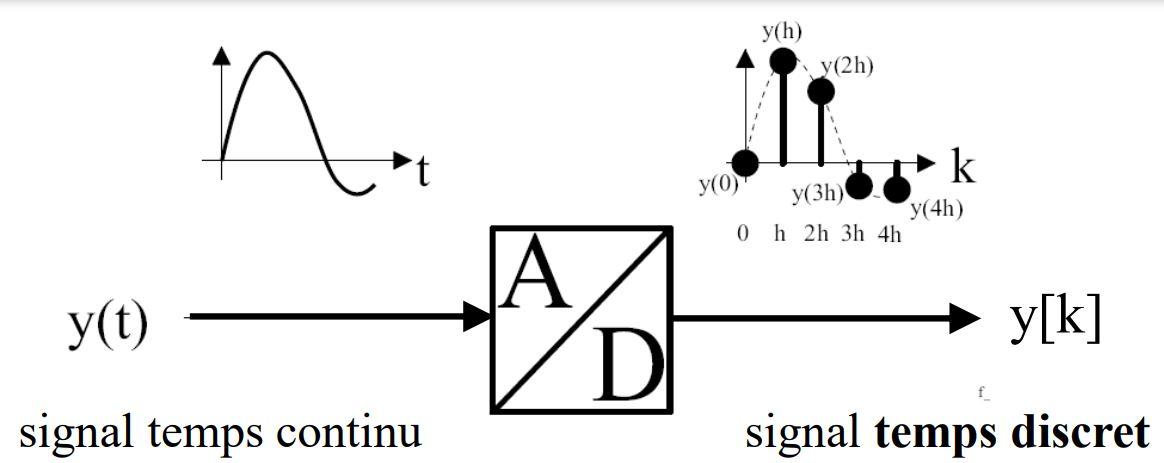
\includegraphics[width = 0.35\textwidth]{img/echantillonage.JPG}
    avec $y[k] = y(k \cdot h)$
\end{center}


Il doit être choisi afin d'éviter les variations trop brutales.

$ h = T_{reg}/20 \; ... \; T_{reg}/10$


\formdesc{Inventaire des retards}

L‘étude « quasi temps-continu » est une première approche pour 
l’analyse et la synthèse approximative d’un système de régulation 
numérique.
Elle est basée sur l’inventaire des retards incontournables que 
possède une boucle de régulation numérique.

Retard du temps de calcul : $T_{cal} < \cfrac{h}{2}$

Retard du bloqueur d'ordre 0 : $T_{rec} \approx \cfrac{h}{2}$

\vspace{3mm}

Retard des conversions :

$T_{convAD} \approx T_{convAD} \approx \cfrac{h}{100} ... \cfrac{h}{10} $


\vspace{2mm}


\vspace{0.5cm}
% Defining string as labels of certain blocks.
\newcommand{\suma}{\Large$+$}
\newcommand{\inte}{$\displaystyle \int$}
\newcommand{\derv}{\huge$\frac{d}{dt}$}

\resizebox{.49\textwidth}{!}{
    \begin{tikzpicture}
        \begin{small} 
            \bXInput{E}
            \bXBloc[4]{algo}{Algo.}{E}
            \bXLink[$w(k)$]{E}{algo}
            \bXBloc[4]{conv1}{D/A}{algo}
            \bXLink[$u(k)$]{algo}{conv1}
            \bXBloc[4]{sys}{Sys.regl.}{conv1}
            \bXLink[$u(t)$]{conv1}{sys}
            \bXOutput[4]{S}{sys}
            \bXLink[$y(t)$]{sys}{S}
            \bXBranchy[4]{S}{U}
            \bXBlocr[12.1]{conv2}{A/D}{U}
            \bXLinkyx{sys-S}{conv2}
            \bXLinkxy[$y(k)$]{conv2}{algo}      
        \node[draw] at (4.8,-2.5) { Retard total : $T_r  =  T_{cal} + T_{convAD} + T_{convAD} + T_{rec} \approx h $};   
        \draw [-latex,red,thick] (3.5,-2.3) to [out=90,in=330] (algo);
        \draw [-latex,blue,thick] (5.3,-2.3) to [out=90,in=320] (conv2);
        \draw [-latex,green!50!black,thick] (6.5,-2.3) to [out=90,in=310] (conv1);
        \draw [-latex,teal!80!purple,thick] (8,-2.3) to [out=90,in=330] (conv1);   
    \end{small}
    \end{tikzpicture}
}



\vspace{3mm}

Ce qui est approximable avec un retard pur par : 

\vspace{3mm}

\underline{Approximations du retard}

\begin{enumerate}
    \item Retard analogique (régime harmonique) :
    
        $e^{-j \omega T_r} = e^{j\varphi}$ avec $\varphi = - \omega T_r$

        $|e^{-j\omega T_r}| = 1$

        $arg(e^{-j\omega T_r}) = -T_r \cdot \omega$

    \item diagramme de Bode du retard analogique exact : 
        \begin{enumerate}
            \item système d'ordre 1 : 
            
                $e^{-j\omega T_r}  \approx \cfrac{1}{1+T_r\cdot j\omega}$

            \item Padé : 
                
                $e^{-j\omega T_r}  \approx \cfrac{1-\cfrac{T_r}{2}j\omega}{1+\cfrac{T_r}{2}j\omega}$

            Exact pour le module (1), mais pas pour la phase !

        \end{enumerate}
\end{enumerate}


\hformbar

\newpage

\formdesc{Rappel Nyquist}

\begin{enumerate}
    \item Condition de stabilité en boucle fermée basée sur un critère en boucle ouverte !
    \item Outil important pour l‘analyse des systèmes réglés, marge de gain $A_m$ , marge de phase $\varphi_m$.
    \item Outil important pour la synthèse des systèmes réglés, choix de $K_p$ pour obtenir $\varphi_m$ souhaitée.
\end{enumerate}

$\varphi_m = arg(G_o(j\omega_{co}))- (-\pi)$ \quad [rad]

\vspace{3mm}

$A_{m,dB} = -|G_o(j\omega_{\pi})| $\quad  [dB]

\vspace{3mm}

\formtitle{Liens entre la boucle ouverte et la boucle fermée} 

bande passante à -3 dB en boucle fermée $\omega_{bp} \approx$ pulsation de coupure en boucle ouverte $\omega_{co}$

$\omega_{bande,passante} = \omega_{co}$

Pulsation de coupure en b.o. $\omega_{co} \Leftrightarrow $ rapidité en b.f

\hformbar

\formdesc{Compensation du pôle dominant}

\begin{enumerate}
    \item Améliorer la dynamique, c-à-d rendre la boucle fermée plus rapide
    \item Faciliter les calculs
\end{enumerate}

\formtitle{Zéros libres du régulateur PI, PD, PID} 


\vspace{2mm}

\underline{PI :}

\vspace{2mm}

{\noindent$G_c(s) = K_p \cfrac{1+T_i \cdot s}{T_i \cdot s} \rightarrow$}

\begin{wrapfigure}[2]{r}{0.25\textwidth}
    \begin{center}
        \vspace{-3.7cm}
        \begin{tikzpicture}[]
            \tikzmath{
            coordinate \x;
            \x1 = (-1.5,0);
            }
            \draw[->] (-2,0) -- (1,0) node [anchor=west] {$R$};
            \draw[->] (0,-0.5) -- (0,0.5) node [anchor=south] {$Img$};
            \draw[thick] (\x1) circle (4pt) node[above=0.2cm] {$Z = -\cfrac{1}{T_i}$};
        \end{tikzpicture}
    \end{center}
  \end{wrapfigure}

  \vspace{10mm}

\underline{PD :}

\vspace{2mm}

{\noindent$G_c(s) = K_p (1+T_d \cdot s) \rightarrow$}

\begin{wrapfigure}[2]{r}{0.25\textwidth}
    \begin{center}
        \vspace{-3.5cm}
        \begin{tikzpicture}[]
            \tikzmath{
            coordinate \x;
            \x1 = (-1.5,0);
            }
            \draw[->] (-2,0) -- (1,0) node [anchor=west] {$R$};
            \draw[->] (0,-0.5) -- (0,0.5) node [anchor=south] {$Img$};
            \draw[thick] (\x1) circle (4pt) node[above=0.2cm] {$Z = -\cfrac{1}{T_d}$};
        \end{tikzpicture}
    \end{center}
  \end{wrapfigure}

  \vspace{10mm}


\underline{PID :}

\vspace{2mm}

{\noindent$G_c(s) = K_p \cfrac{1+T_i \cdot s+T_i \cdot T_d \cdot s^2}{T_i \cdot s}$}

\vspace{2mm}

zéros réels si : $T_i > 4\cdot T_d$

    \begin{center}
        \tikzset{cross/.style={cross out, draw=black, minimum size=2*(#1-\pgflinewidth), inner sep=0pt, outer sep=0pt},
        cross/.default={4pt}}
        \begin{tikzpicture}[]
            \tikzmath{
            coordinate \x;
            \x1 = (-5,0);
            \x2 = (-2,0);
            \x3 = (0,0);
            }
            \draw[->] (-6,0) -- (1,0) node [anchor=west] {$R$};
            \draw[->] (0,-0.5) -- (0,0.5) node [anchor=south] {$Img$};
            \draw[thick] (\x3) node[cross] {};
            \draw[thick] (\x2) circle (4pt) node[above=0.2cm] {$Z_1 \approx -\cfrac{1}{T_i}$};
            \draw[thick] (\x1) circle (4pt) node[above=0.2cm] {$Z_2 \approx -\cfrac{1}{T_d}$};
        \end{tikzpicture}
    \end{center}

    La compensation se fait en appliquant la règle suivante : 
    
    Zéro du régulateur = Pôle de système à régler

    \tikzset{cross/.style={cross out, draw=black, minimum size=2*(#1-\pgflinewidth), inner sep=0pt, outer sep=0pt},
cross/.default={4pt}}

\tikzset{ % this style creates an arrow like the one you draw in the middle of a path
   ->-/.style={decoration={markings,mark=at position 0.5 with {\arrow{Straight Barb}}},
               postaction={decorate}}
}
%default radius will be 1pt. 
\begin{tikzpicture}[]
    \tikzmath{
    coordinate \x;
    \x1 = (-2,0);
    \x2 = (-1,0);
    \x3 = (-5,0);
    \x4 = (-3.5,0);
    \x5 = (-1,0);
    }
    \draw[->] (-6,0) -- (1,0) node [anchor=west] {$R$};
    \draw[->] (0,-0.5) -- (0,0.5) node [anchor=south] {$Img$};

    \draw[thick] (\x1) node[cross] {};
    \draw[] (\x1) node[above=0.2cm] {$S_{a2}$};
    \draw[thick] (\x2) node[cross] {};
    \draw[] (\x2) node[above=0.2cm] {$S_{a1}$};
    \draw[thick] (\x4) node[cross] {};
    \draw[] (\x4) node[above=0.2cm] {$S_{a3}$};

    \draw[thick] (\x3) circle (4pt) node[above=0.2cm] {$Z_{a1} $};

    \draw[thick] (\x5) circle (4pt) node[below=0.2cm] {$Z_{c1} $};
    
\end{tikzpicture}


\hformbar

\newpage

\formdesc{schéma et FTZ dérivateur}


\begin{center}
    \begin{tikzpicture}[scale=0.5]
            \bXInput{E}
            \bXBloc[4]{sys}{$\cfrac{d}{dt}$}{E}
            \bXLink[$u(t)$]{E}{sys}
            \bXOutput[4]{S}{sys}
            \bXLink[$y(t)$]{sys}{S}
    \end{tikzpicture}
\end{center}

\vspace{-3mm}

\formtitle{Méthode des séquentes : }  

\vspace{3mm}

{\hfill $y[k] = \cfrac{du}{dt} \approx \cfrac{\Delta u}{\Delta t}= \cfrac{u[k]-u[k-1]}{h}$ \hfill}

\vspace{3mm}

\formtitle{schéma bloc numérique :}   

\begin{center}
    \begin{tikzpicture}
        \begin{small} 
            \bXInput{E}
            \bXBloc[4]{retard}{$Z^{-1}$}{E}
            \bXLink[$\text{u[k]}$]{E}{retard}
            \bXCompSum[6]{comp}{retard}{}{+}{-}{}
            \bXLink[$\text{u[k-1]}$]{retard}{comp}
            \bXBloc[4]{div}{$\cfrac{1}{h}$}{comp}
            \bXLink[]{comp}{div}
            \bXOutput[4]{S}{div}
            \bXLink[$\text{y[k]}$]{div}{S}
            \bXReturn{E-retard}{comp}{}
            \node at (E-retard)[circle,fill,inner sep=1pt,below=0.225cm]{};
        \end{small}
    \end{tikzpicture}
    $G_d(Z) = (1-z^{-1}) \cdot \cfrac{1}{h} = \cfrac{Z-1}{hZ}$
\end{center}

\hformbar

\formdesc{schéma et FTZ intégrateur}

\begin{center}
    \begin{tikzpicture}
            \bXInput{E}
            \bXBloc[4]{sys}{\huge$\int$}{E}
            \bXLink[$u(t)$]{E}{sys}
            \bXOutput[4]{S}{sys}
            \bXLink[$y(t)$]{sys}{S}
    \end{tikzpicture}
\end{center}

\vspace{-3mm}

\formtitle{Méthode des rectangles : }   

\vspace{3mm}
{\hfill $y[k+1] = y[k] + h \cdot u[k]$\hfill} 

\vspace{3mm}

\underline{schéma bloc numérique :}   

\begin{center}
    \begin{tikzpicture}
        \begin{small} 
            \bXInput{E}
            \bXBloc[4]{h}{$h$}{E}
            \bXSumb[6]{comp}{h}
            \bXBloc[4]{ret}{$Z^{-1}$}{comp}
            \bXOutput[4]{S}{ret}
            \bXLink[$\text{u[k]}$]{E}{h}
            \bXLink[]{h}{comp}
            \bXLink[$\text{y[k+1]}$]{comp}{ret}
            \bXLink[$\text{y[k]}$]{ret}{S}
            \bXReturn{ret-S}{comp}{}
            \node at (ret-S)[circle,fill,inner sep=1pt,below=0.225cm]{};
        \end{small}
    \end{tikzpicture}
    $G_i(Z) = \cfrac{h \cdot z^{-1}}{1 - z^{-1}}= \cfrac{h}{Z-1}$
\end{center}

\hformbar

\newpage

\formdesc{Méthode de "Tustin" (trapèzes) : }   

\underline{Idée de la méthode de numérisation de "Tustin" :}

pour une fonction de transfert analogique quelconque, 
remplacer chaque occurrence de s par l'expression en z ci-dessous

\vspace{3mm}

$y[k] = y[k-1] + h \cdot \cfrac{u[k-1]+u[k]}{2}$

\vspace{3mm}

$G_i(Z) = \cfrac{h \cdot (z^{-1}+1)}{2(1 - z^{-1})} \approx \cfrac{1}{S}$


$G_d(Z) = \cfrac{2(1 - z^{-1})}{h \cdot (z^{-1}+1)} \approx S$




\hformbar
\formdesc{Lieu des poles(Root locus)}

\footnotesize Outil important permettant la synthèse de systèmes réglés : 

pôles complexes conjugués :

{\hfill $s_{1,2} = -\delta \pm j\omega $\hfill}

Réponse indicielle :

{\hfill $g(t) = e^{-\delta \cdot t} \cdot sin(\omega t) $\hfill}

Rappel (formulaire régulation automatique) : 

{\hfill $T_{reg} = \cfrac{3}{\delta} = \cfrac{-3}{\mathbb{R}(s_f)}$\hfill}\vspace{3mm}

Règles de tracer du lieu des pôles (L.d.P) :
\begin{enumerate}
    \item L.d.P a n branches = degré du dénominateur 
    \item L.d.P a M branches = degré du numérateur
    \item L.d.P symétrique par l'axe $\mathbb{R}$
    \item Points de départ à $K_p = 0$
    \item Points de fin à $K_p = \infty$
    \item $d = n-m$ branches restante partent en asymptote infinie, où d correspond au degré relatif de la B.O\\ les asymptotes forment des étoiles régulières
    \item Tout point de l'axe réel situé à gauche d'un nombre impair de pôles et de zéros réels fait partie du lieu
\end{enumerate}

\tikzset{cross/.style={cross out, draw=black, minimum size=2*(#1-\pgflinewidth), inner sep=0pt, outer sep=0pt},
cross/.default={4pt}}

\tikzset{ % this style creates an arrow like the one you draw in the middle of a path
   ->-/.style={decoration={markings,mark=at position 0.5 with {\arrow{Straight Barb}}},
               postaction={decorate}}
}
%default radius will be 1pt. 
\begin{tikzpicture}[]
    \tikzmath{
    coordinate \x;
    \x1=(-2,0);
    \x2=(0,0);
    \x3=(-2.5,0);
    \x4 = (-3,0);
    \x5 = (-1,0);
    }
    
    \draw[help lines,dashed] (-5.5,-1.5) grid (0.5,1.5);
    \draw[->] (-6,0) -- (1,0) node [anchor=west] {$R$};
    \draw[->] (0,-1.5) -- (0,1.5) node [anchor=south] {$Img$};
    \draw[->-,red,thick] (\x1) -- (\x5);
    \draw[->-,red,thick] (\x5) arc (0:180:1);
    \draw[->-,red,thick] (\x4) -- (\x3);
    
    \draw[->-,blue,thick] (\x2) -- (\x5);
    \draw[->-,blue,thick] (\x5) arc (0:-180:1);
    \draw[->-,blue,thick] (\x4) -- (-6,0);
    \draw (\x1) node[cross] {};
    \draw (\x2) node[cross] {};
    \draw (\x3) circle (4pt);
    
\end{tikzpicture}


\hformbar



\formdesc{Transformé en Z}

\begin{figure}[H]
    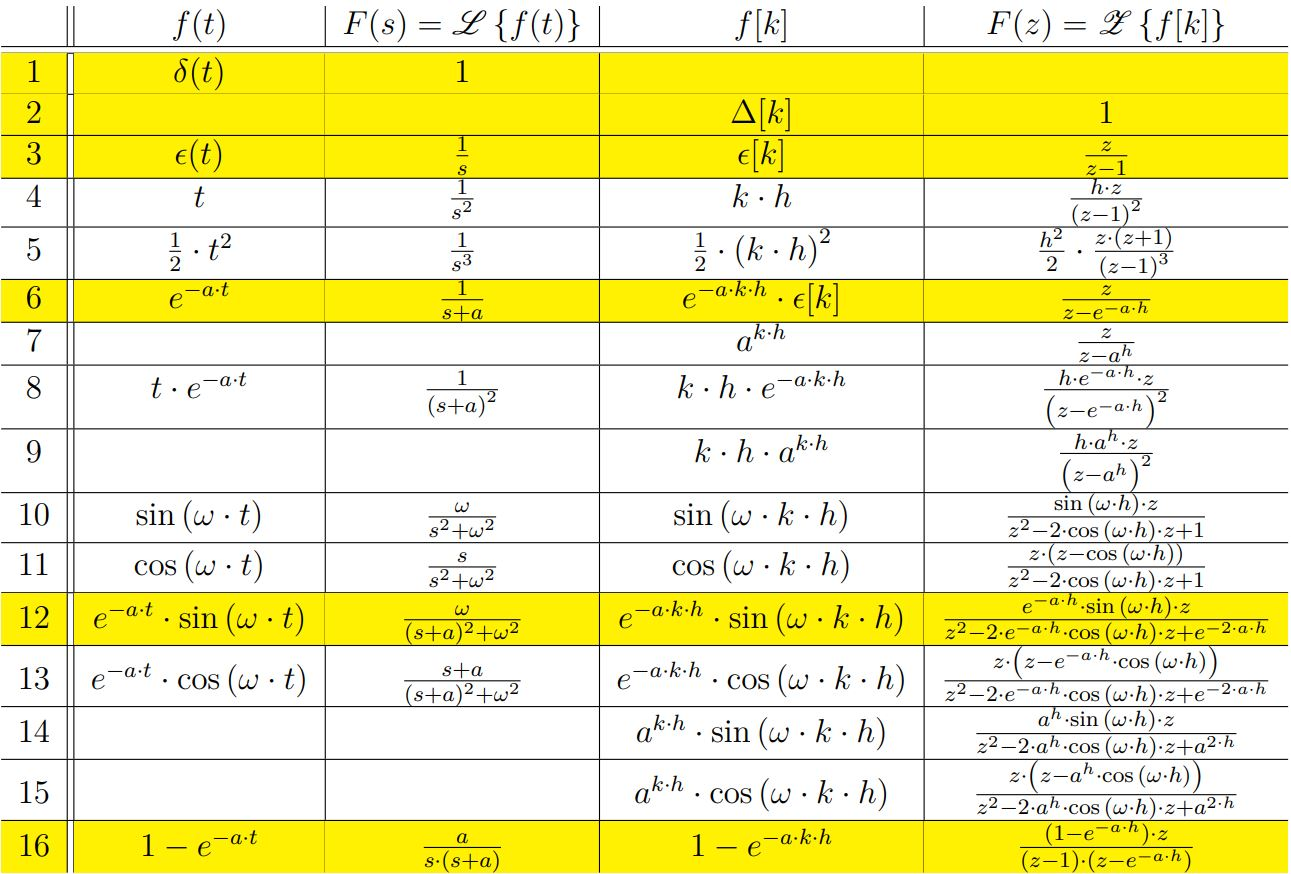
\includegraphics[width  = 1\textwidth]{img/Tranforme_en_Z.JPG}
    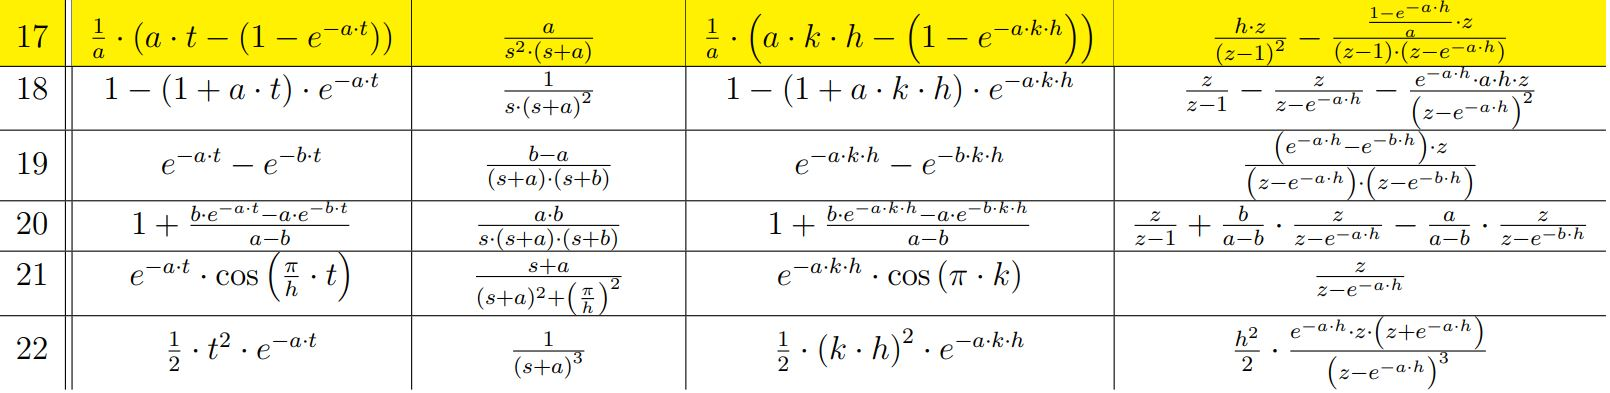
\includegraphics[width  = 1\textwidth]{img/Tranforme_en_Z2.JPG}
\end{figure}

\formdesc{Modèle échantillonné du système à régler}

\underline{Boucle fermé hybride }

Parie analogique et numérique

\begin{center}
    \begin{tikzpicture}
        \begin{small} 
            \bXInput{E}
            \bXBloc[4]{D_A}{$D/A$}{E}
            \bXBloc[4]{Ga}{$G_a(s)$}{D_A}
            \bXBloc[4]{A_D}{$A/D$}{Ga}
            \bXOutput[4]{y}{A_D}

            \bXLink[$u(k)$]{E}{D_A}
            \bXLink[$u(t)$]{D_A}{Ga}
            \bXLink[$y(t)$]{Ga}{A_D}
            \bXLink[$y(k)$]{A_D}{y}
        \end{small}
    \end{tikzpicture}
\end{center}

Ce problème peut être résolu en utilisant le modèle échantillonné $H(z)$ dans les calculs dans le domaine en z.

\begin{center}
    \begin{tikzpicture}
        \begin{small} 
            \bXInput{E}
            \bXBloc[10]{H}{$H(z)$}{E}
            \bXOutput[10]{y}{H}

            \bXLink[$U(z)$]{E}{H}
            \bXLink[$Y(z)$]{H}{y}
        \end{small}
    \end{tikzpicture}
\end{center}


$H(z) = \cfrac{Y(z)}{U(u)}= \cfrac{z-1}{z} \cdot \mathcal{Z}\biggl\{ \mathcal{L}^-1\biggl( \cfrac{G_a(s)}{s}\biggr)\bigg|_{t = k\cdot h}\biggr\}$

Exemple :

\begin{enumerate}
    \item $\cfrac{G_a(s)}{s} = \cfrac{G_a(s)}{s(s-p_a)}$
    \item $\mathcal{L}^-1\biggl(\cfrac{G_a(s)}{s}\biggr) = \cfrac{ka}{-pa} \cdot 1-e^{p_a \cdot t}$ (Réponse indicielle)
    \item $\cfrac{ka}{-pa} \cdot 1-e^{p_a \cdot t}\bigg|_{t = k\cdot h} = \cfrac{ka}{-pa} \cdot 1-e^{p_a\cdot k\cdot h}$
    \item $\mathcal{Z}\biggl\{ \cfrac{ka}{-pa} \cdot 1-e^{p_a\cdot k\cdot h}  \biggr\} = \cfrac{ka}{-pa} \cfrac{z\cdot(1-e^{pa \cdot h})}{(z-1)\cdot(Z-e^{pa \cdot h})}$
    \item $\cfrac{z-1}{z} \mathcal{Z}\biggl\{...\biggr\} = \cfrac{ka}{-pa} \cfrac{1-e^{pa \cdot h}}{Z-e^{pa \cdot h}}$
\end{enumerate}

Donc les relations entre le plan s et Z sont : 

$p_n = e^{p_a\,h}$

$z = e^{s \, h}$

\underline{Propriétés du "modèle échantillonné"}
\begin{enumerate}
    \item pôles analogique se transforme selon $z = e^{s \, h}$
    \item Le gain  statique est préservé : $H(z = 1) = G_a(s = 0)$
    \item $H(z) $est linéaire en $G_a(s)$ : $G_{a1}(s) + G_{a2 }(s) \Leftrightarrow H_1(z) + H_2(z)$ Pas valable pour le produit 
    \item Un retard pur de N période coté analogique donne lieu à un facteur z dans la modèle échantillonné $e^{-H\,h}\Leftrightarrow z^N$
\end{enumerate}

\underline{Calcul du modèle échantillonné du système à régler}

le calcul se fait avec la réponse impulsionnelle.

$u[k] = \Delta[k]$ (Dirac numérique)

$\mathcal{L}\bigg(u(t) = \varepsilon(t) - \varepsilon(t-h)\bigg) = \cfrac{1}{s} - \cfrac{1}{s} \cdot e^{-h\,s} = U(s) $

Exemple sans retard : 

$u[k] = \{1,0,0,0\} \rightarrow y[k] = \{0,h,h,h\}$ (Intégrateur)

$y[k] =h \cdot \varepsilon[k-1] \rightarrow \mathcal{Z}(y) = H(z) = h \cdot z^{-1} \cfrac{z}{z-1} = \cfrac{h}{z-1} $

Exemple avec retard h/2 : 


$u[k] = \{1,0,0,0\} \rightarrow y[k] = \{0,h/2,h,h\}$ (Intégrateur)

$y[k] =h \cdot \varepsilon[k-2] + \cfrac{h}{2} \Delta[k-1]$

$\mathcal{Z}(y) = H(z) = h \cdot z^{-2} \cfrac{z}{z-1} + \cfrac{h}{2} \cdot z^{-1} = h\cfrac{1+\cfrac{1}{2}(z-1)}{z(z-1)} $


\underline{Avantages du modèle échantillonné}

\begin{itemize}
    \item Analyse et synthèse complètement en z
    \item Pas besoin de traiter le système hybride.
    \item Calculs exacts contrairement à l'inventaire des retards.
\end{itemize}

\underline{Correspondance entre le plan de s et le plan de z}

\begin{itemize}
    \item Le plan de z est "moins parlant" que le plan de s
    \item Beaucoup de caractéristiques, p.ex. taux d'amortissement sont définies en s
    \item Pour la synthèse par "placement de pôles", d'abord choisir les pôles en s et calculer les pôles en z correspondants
    \item Pour l'analyse, d'abord calculer les pôles en z, puis calculer les pôles en s correspondants en utilisant la fonction réciproque (log)
\end{itemize}

\underline{Avec ma calculatrice nulle}

$s = delta + j\omega$

$z = e^{s\,h} = e^{delta\,h + j\omega\,h} = 1\angle j\omega h $

$s = \cfrac{ln(z)}{h} = \cfrac{1}{h} \bigg(ln(|z|)+ln(e^{j\,arg(z)})\bigg) $

$=\cfrac{1}{h} \bigg(ln(|z|)+j\,arg(z)\bigg)$

\begin{figure}[H]
    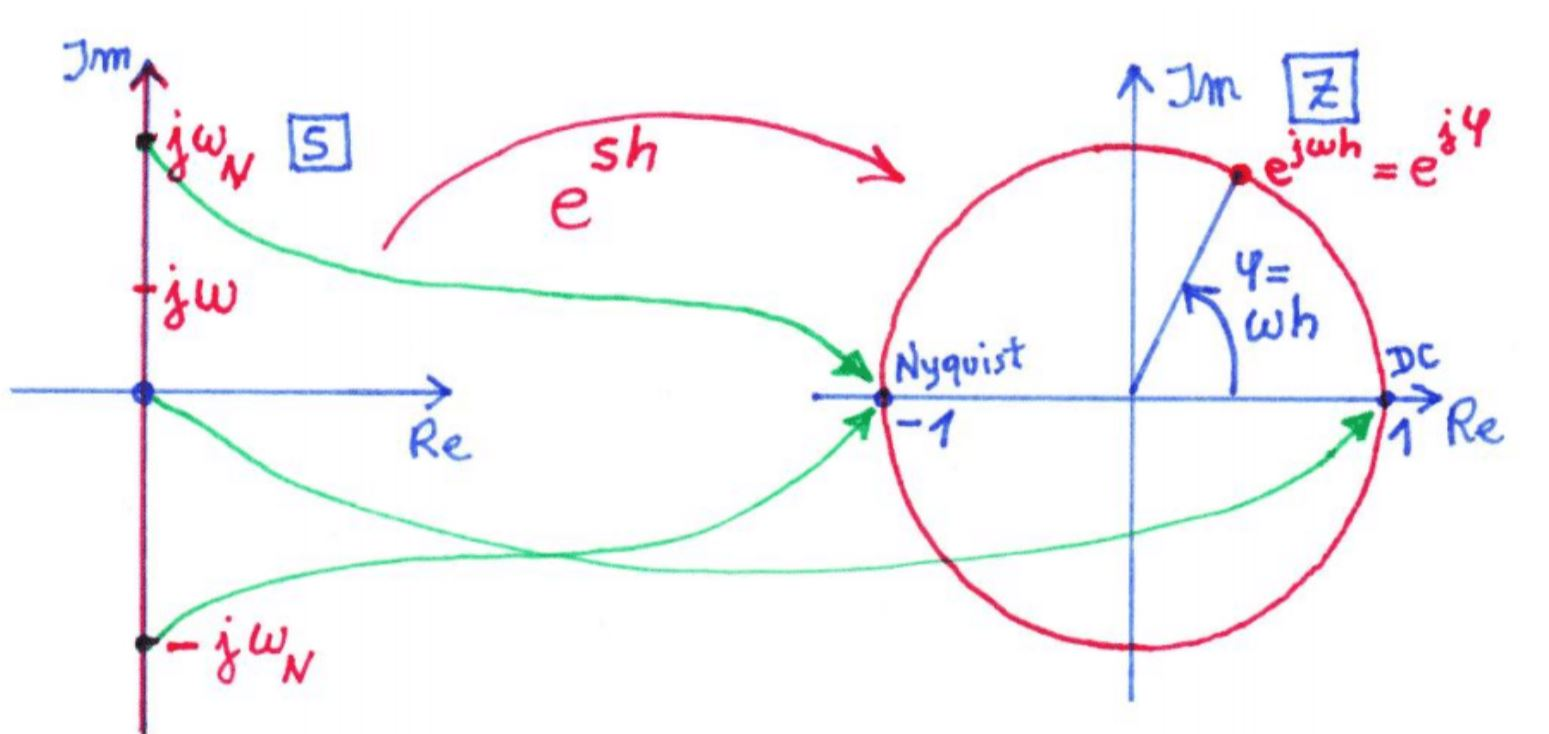
\includegraphics[width  = 0.48\textwidth]{img/ZtoS.JPG}
\end{figure}




\formdesc{Régime harmonique }   

\underline{Rappel :}

\begin{center}
    \begin{tikzpicture}
        \begin{small} 
            \bXInput{E}
            \bXBloc[10]{H}{$G_a(s)$}{E}
            \bXOutput[10]{y}{H}

            \bXLink[$u(t) = U\cdot sin(wt)$]{E}{H}
            \bXLink[$y(t) = Y \cdot sin(wt+\varphi)$]{H}{y}
        \end{small}
    \end{tikzpicture}
\end{center}

donc : $y = |G_a(jw)| \cdot U\;; \;\varphi = arg(G_a(jw))$

La représentation du régime amorti établi,
la fonction de transfert analogique est évaluée sur l'axe imaginaire.
$s = j\omega$ 

en numérique cela donne : 

$u[k] = U\cdot sin(w\,k\,h)$

$y[k] = Y\cdot sin(w\,k\,h+\varphi)$

donc : $y = |G_n(e^{jwh})| \cdot U\;; \;\varphi = arg(G_n(e^{jwh}))$


La représentation du régime amorti établi,
la fonction de transfert numérique est évaluée sur le cercle unité.

Par conséquent, 

$G_a(e^{jwh}) = G_n(z = e^{jwh})$


%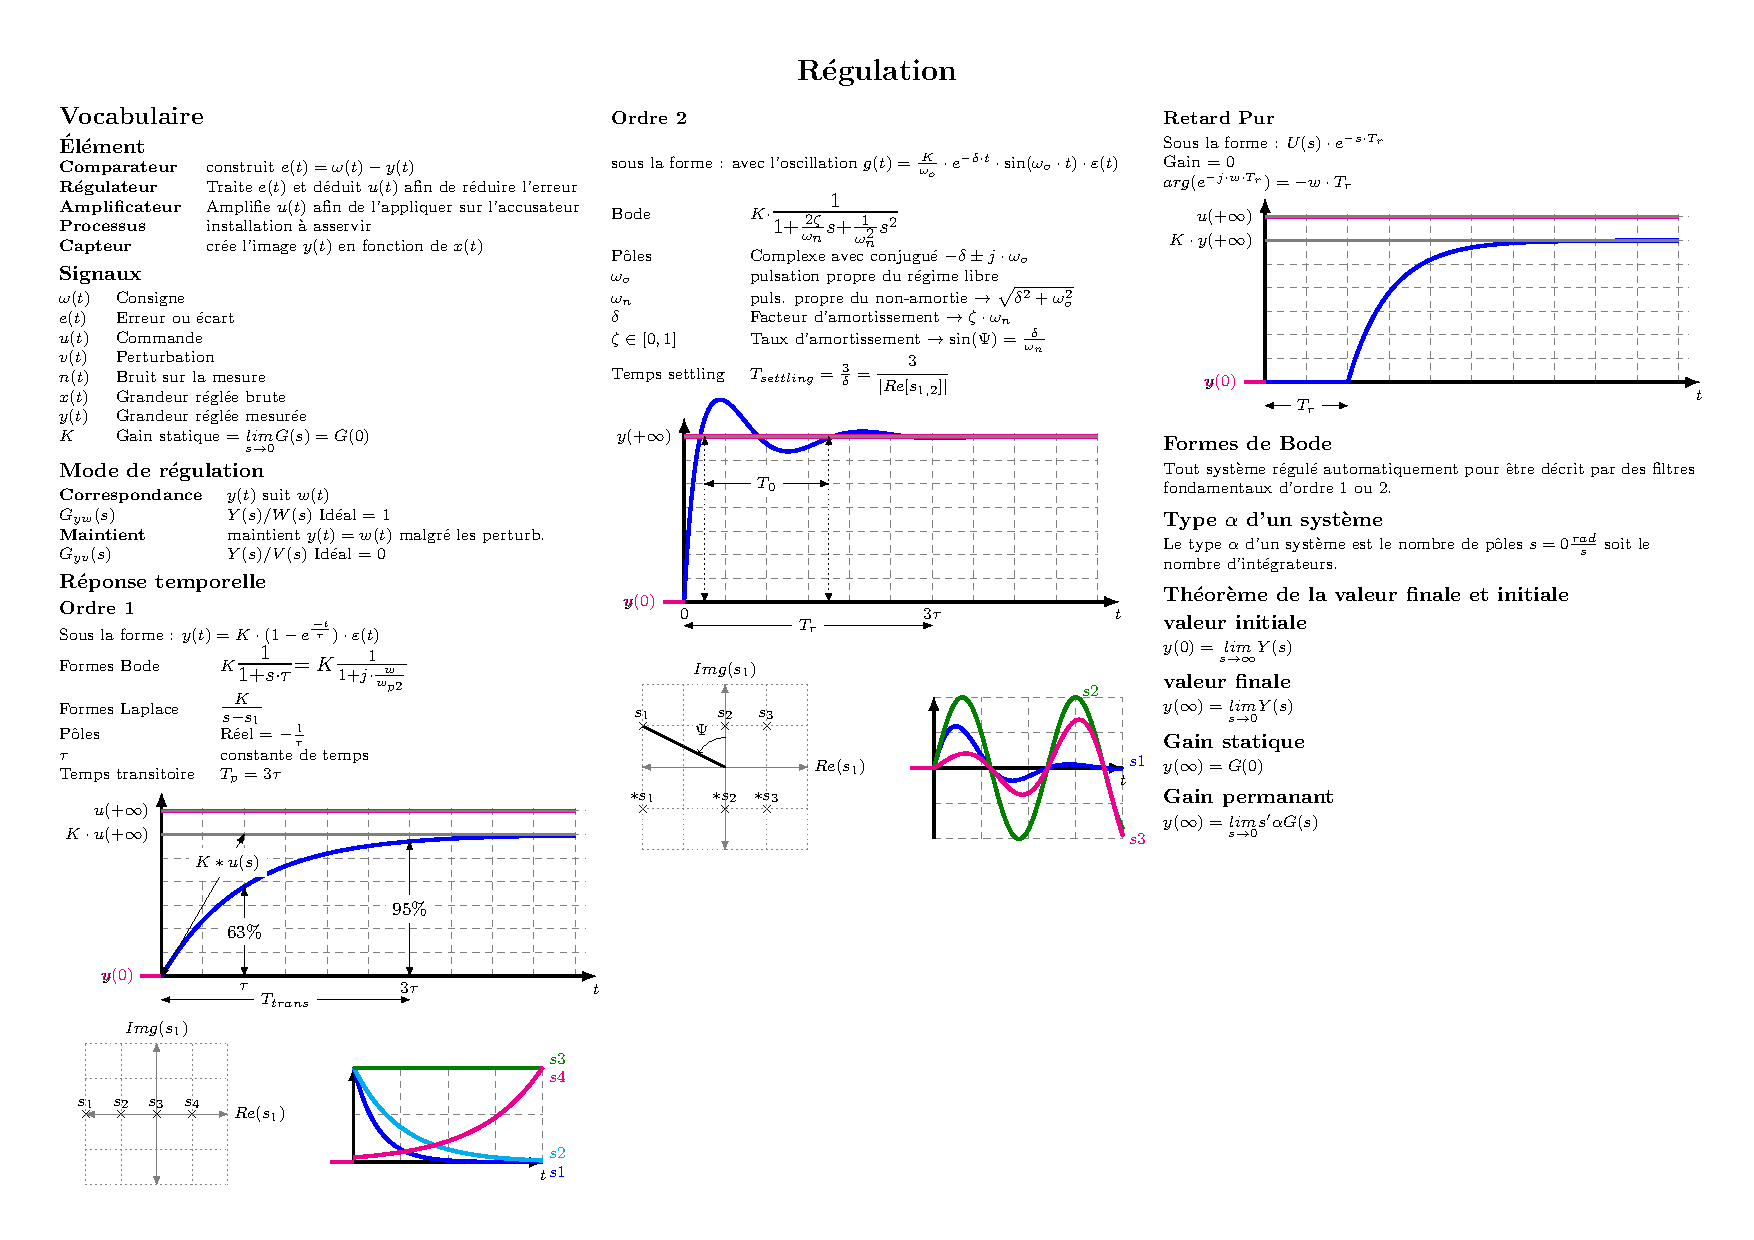
\includepdf[pages=-]{img/cheat.pdf}

\end{document}